% !TEX root = ../Abschlussbericht_Schimmeliger_Keller.tex
%%
%%  Hochschule für Technik und Wirtschaft Berlin --  Projektabschlussbericht
%%
%% Kapitel 4 - Praktische Umsetzung
%%
%%

\chapter{Praktische Umsetzung} \label{Praktische Umsetzung}
\section{Verwendete Hardware} \label{Hardware}
\subsection{LoPy4-Development-Board} \label{LoPy4}



\subsection{DHT Sensormodul} \label{DHT}

Bei dem verwendeten Sensor handelt es sich um einen sog. DHT Sensor. Diesen gibt es in zwei verschiedenen Ausführungen, DHT11 und DHT22, wobei sich diese im auswertbaren Messbereich, der Messgenauigkeit und im Preis unterscheiden.

\begin{adjustwidth}{-1in}{-1in}% adjust the L and R margins by -1 inch
	\begin{center}
	
	        \begin{tabular}{ccc}
			\toprule
			 & \textbf{DHT11} & \textbf{DHT22}\\

			\midrule
			Betriebsspannung & \multicolumn{2}{c}{3 \dots 5 V DC}\\
			Stromverbrauch & \multicolumn{2}{c}{max. 2,5 mA während der Konvertierung}\\
			Temperaturbereich & -20\dots 60 °C & -40\dots 80 °C  \\
			Temperatur Genauigkeit & ± 2,0 °C & ± 0,5 °C\\
			Feuchtigkeit Messbereich & 20\%\dots90\% RH & 0\%\dots99,9\% RH\\
			Feuchtigkeit Genauigkeit & ± 5,0\% RH & ± 2\dots5\%\\
			Abtastrate & 1 Hz & 0,5 Hz \\

			\midrule
			Preis (bei reichelt elektronik) & 1,80 € & 6,80 €\\

			\bottomrule
	
	        \end{tabular}
		\label{}
		\captionof{table}{Vergleich DHT11 zu DHT22} \label{tab:vergleichDHT} 
	\end{center}
\end{adjustwidth}

Anzumerken ist noch, dass der DHT22 Sensorungefähr das doppelte Volumen des DHT11 Sensors hat. Interessant ist auch, dass der DHT11 Sensor ungefähr doppelt so häufig angesprochen werden kann, was vermutlich auf seiner weniger komplexen Schaltung beruht.\\
Für die meisten Anwendungsfälle würde wahrscheinlich ein DHT11 Sensor (oder mehrere parallel geschaltete DHT11 Sensoren) ausreichen, um ein weitgehend zuverlässiges Ergebnis zu erhalten.



\begin{center}
	\begin{figure}[h]
	 
	 \noindent\makebox[\textwidth]{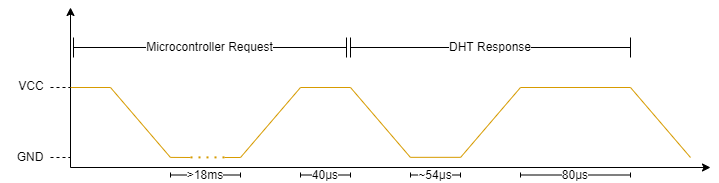
\includegraphics[width=0.9\textwidth]{pictures/dht_kommunikation1}}
	 \caption[DHT Kommunikation]{DHT Kommunikation}
	 \label{fig:dhtkommunikation}
	\end{figure}
\end{center}


\begin{center}
	\begin{figure}[h]
	 
	 \noindent\makebox[\textwidth]{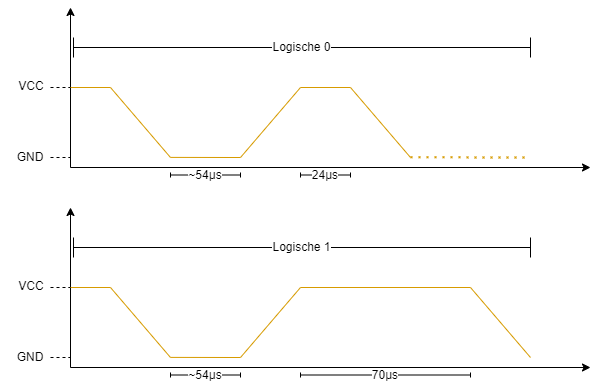
\includegraphics[width=0.9\textwidth]{pictures/dht_kommunikation2}}
	 \caption[DHT Bit Identifikation]{DHT Bit Identifikation}
	 \label{fig:dhtbits}
	\end{figure}
\end{center}




\begin{center}
	\begin{figure}[h]
	 
	 \noindent\makebox[\textwidth]{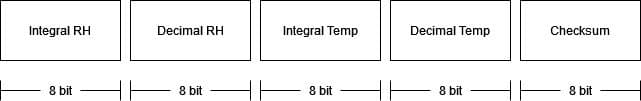
\includegraphics[width=0.7\textwidth]{pictures/dht11_dataframe}}
	 \caption[DHT Paketstruktur]{DHT Paketstruktur}
	 \label{fig:dhtpaketstruktur}
	\end{figure}
\end{center}



\subsection{Restliche Hardware} \label{Restliche Hardware}




\section{Beschreibung der Software} \label{Software}

Für unser Projekt haben wir drei verschiedene, miteinander interagierende Software Komponenten realisiert, welche über eine Schnittstelle (Interface) miteinander kommunizieren. 
Der Vorteil einer solchen Architektur ist, dass die einzelnen Komponenten sich unter umständen wiederverwenden lassen und sich im Idealfall so eine Software modular aufbauen lässt.
Da wir als Programmiersprache ausschließlich Python bzw. Micropython verwendet haben, könnte man argumentieren, dass unsere Software automatisch Modular ist, da sich in der Theorie alle programmierten Komponenten in Python wiederverwenden lassen.
Dies ist aber sehr verallgemeinert gesprochen, da gerade die Programmierung der Mikrocontroller definitiv auch Individualsoftware benötigt, welche sich aber immerhin nicht nur auf einer einzelnen Mikrocontrollerfamilie ausführen funktionieren würde.
Anzumerken ist noch, dass für unsere finale Version des Projektes vermutlich nur eine einzelne Softwarekomponente notwendig wäre.


\subsection{1. Komponente: Sensoransteuerung und der Versand der Daten mittels LoRa(WAN)} \label{Sender}

Für die Programmierung der Mikrocontroller verwenden wir die Programmiersprache Micropython, welche eine schlanke und schnelle Implementation der Programmiersprache Python ist, welche für Mikrocontroller optimiert wurde.

\begin{center}
	\begin{figure}[h]
	 
	 \noindent\makebox[\textwidth]{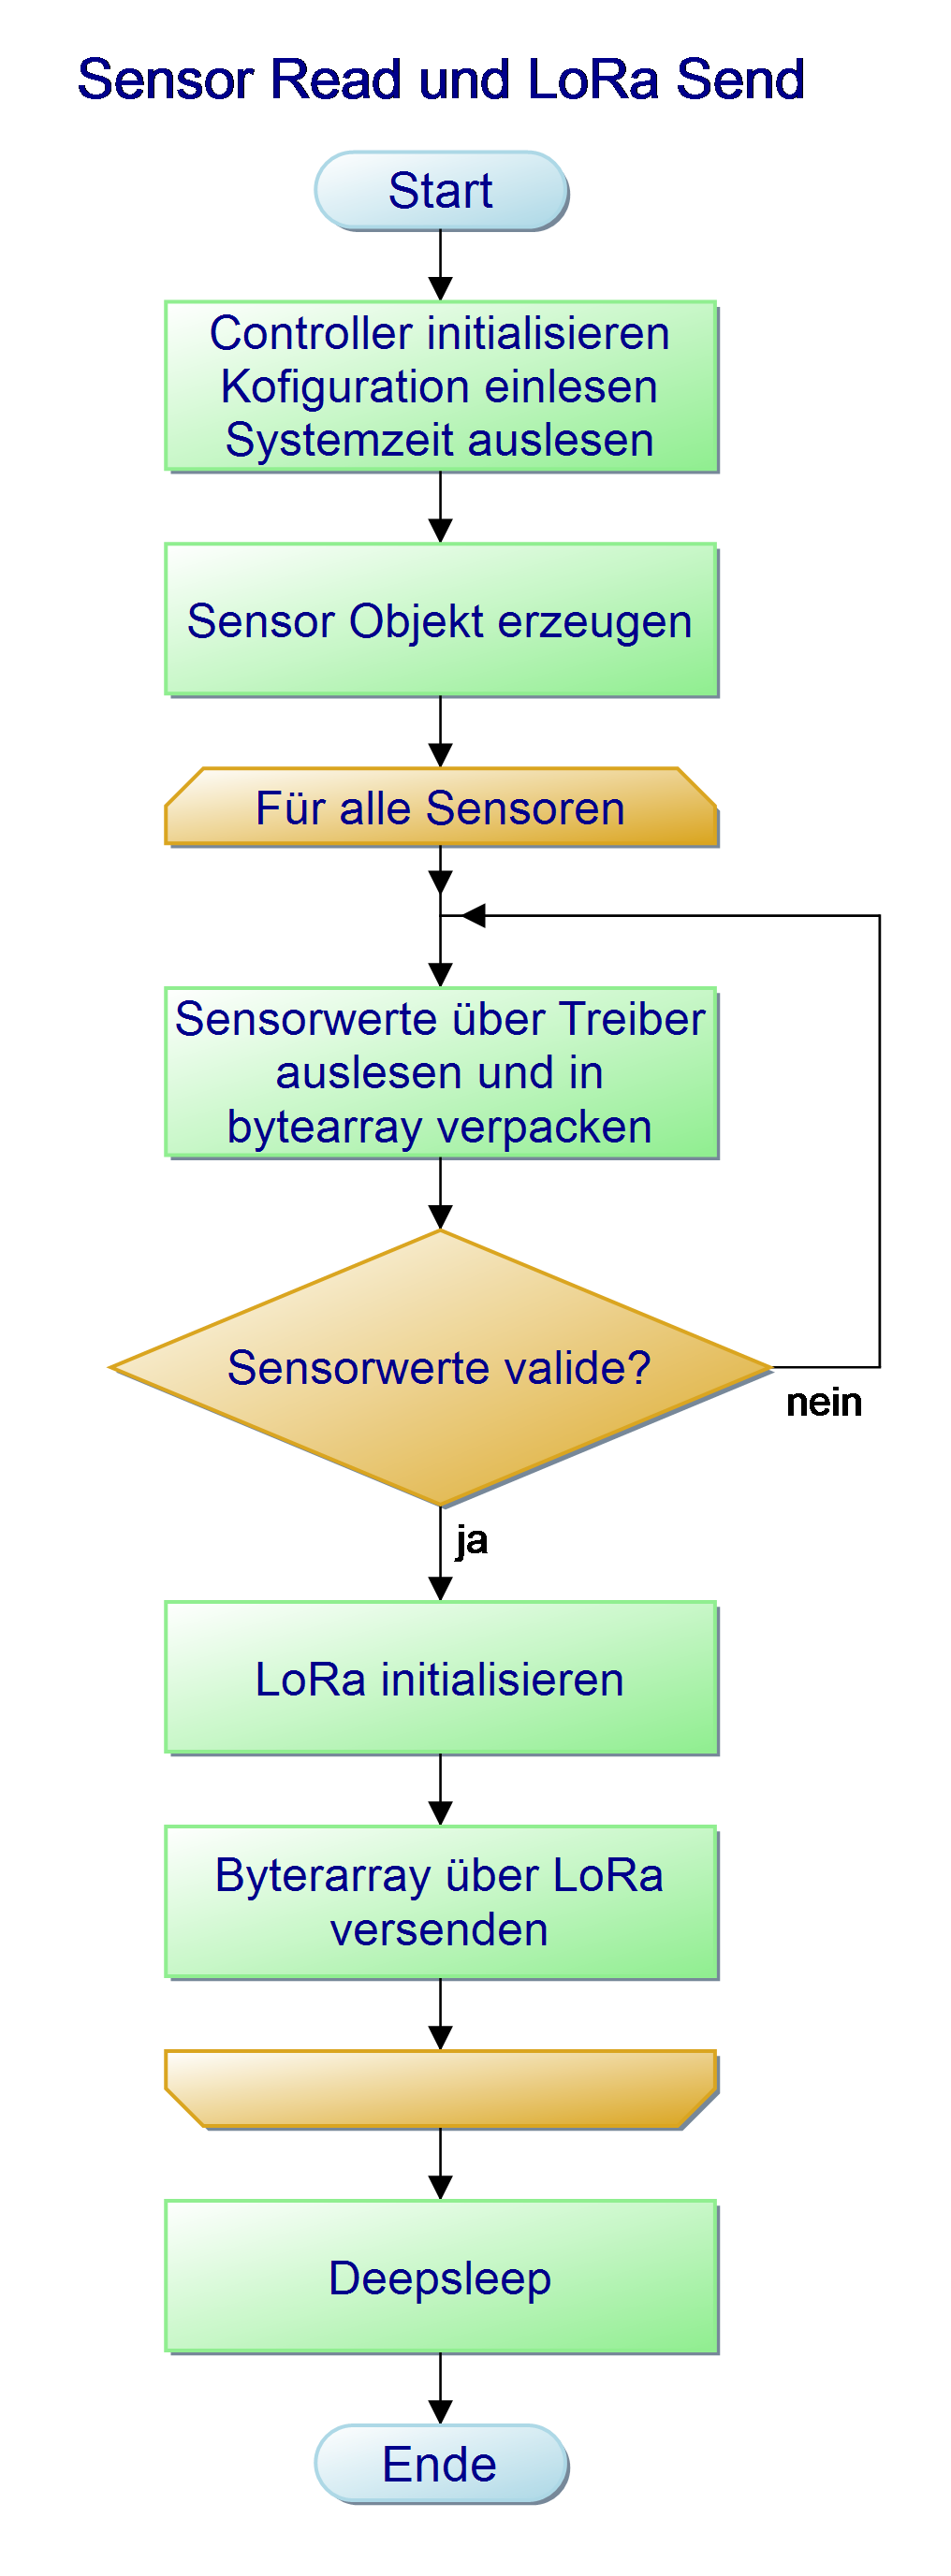
\includegraphics[width=0.4\textwidth]{pictures/sens_read_lora_send}}
	 \caption[PAP komponente 1]{Programm Ablauf: Komponente 1}
	 \label{fig:zeitplanung}
	\end{figure}
\end{center}

\subsection{2. Komponente: Emfangen der Daten und Versand ins Internet} \label{Empfänger}

\ldots

\subsection{3. Komponente: Manuelles abrufen und versenden der veröffentlichten Daten} \label{PubSub}

\ldots


\section{Visualisierung der Sensordaten} \label{Dashboard und Visualisierung}

\ldots


\section{Berechnung der Laufzeit im Batteriebetrieb} \label{Simulation}

\ldots
